%----------------------------------------------------------------------------------------
%	PACKAGES AND OTHER DOCUMENT CONFIGURATIONS
%----------------------------------------------------------------------------------------

\documentclass{article}
\usepackage{xeCJK} %调用 xeCJK 宏包
\setCJKmainfont{STFangsong} %设置 CJK 主字体为 SimSun (宋体)
\usepackage{fancyhdr} % Required for custom headers
\usepackage{lastpage} % Required to determine the last page for the footer
\usepackage{extramarks} % Required for headers and footers
\usepackage[usenames,dvipsnames]{color} % Required for custom colors
\usepackage{graphicx} % Required to insert images
\usepackage{listings} % Required for insertion of code
\usepackage{courier} % Required for the courier font
\usepackage{lipsum} % Used for inserting dummy 'Lorem ipsum' text into the template
\usepackage{booktabs}
\usepackage{multirow}

% Margins
\topmargin=-0.45in
\evensidemargin=0in
\oddsidemargin=0in
\textwidth=6.5in
\textheight=9.0in
\headsep=0.25in

\linespread{1.1} % Line spacing

% Set up the header and footer
\pagestyle{fancy}
\lhead{\hmwkAuthorName\ \hmwkAuthorNumber} % Top left header
\chead{\hmwkClass\ : \hmwkTitle} % Top center head
\rhead{\firstxmark} % Top right header
\lfoot{\lastxmark} % Bottom left footer
\cfoot{} % Bottom center footer
\rfoot{Page\ \thepage\ of\ \protect\pageref{LastPage}} % Bottom right footer
\renewcommand\headrulewidth{0.4pt} % Size of the header rule
\renewcommand\footrulewidth{0.4pt} % Size of the footer rule

\setlength\parindent{0pt} % Removes all indentation from paragraphs

%----------------------------------------------------------------------------------------
%	CODE INCLUSION CONFIGURATION
%----------------------------------------------------------------------------------------

\definecolor{MyDarkGreen}{rgb}{0.0,0.4,0.0} % This is the color used for comments
\lstloadlanguages{Python} % Load Perl syntax for listings, for a list of other languages supported see: ftp://ftp.tex.ac.uk/tex-archive/macros/latex/contrib/listings/listings.pdf
\lstset{language=Python, % Use Perl in this example
        frame=single, % Single frame around code
        basicstyle=\small\ttfamily, % Use small true type font
        keywordstyle=[1]\color{Blue}\bf, % Perl functions bold and blue
        keywordstyle=[2]\color{Purple}, % Perl function arguments purple
        keywordstyle=[3]\color{Blue}\underbar, % Custom functions underlined and blue
        identifierstyle=, % Nothing special about identifiers                                         
        commentstyle=\usefont{T1}{pcr}{m}{sl}\color{MyDarkGreen}\small, % Comments small dark green courier font
        stringstyle=\color{Purple}, % Strings are purple
        showstringspaces=false, % Don't put marks in string spaces
        tabsize=5, % 5 spaces per tab
        %
        % Put standard Perl functions not included in the default language here
        morekeywords={rand},
        %
        % Put Perl function parameters here
        morekeywords=[2]{on, off, interp},
        %
        % Put user defined functions here
        morekeywords=[3]{test},
       	%
        morecomment=[l][\color{Blue}]{...}, % Line continuation (...) like blue comment
        numbers=left, % Line numbers on left
        firstnumber=1, % Line numbers start with line 1
        numberstyle=\tiny\color{Blue}, % Line numbers are blue and small
        stepnumber=5 % Line numbers go in steps of 5
}

% Creates a new command to include a perl script, the first parameter is the filename of the script (without .pl), the second parameter is the caption
\newcommand{\pythonscript}[2]{
\begin{itemize}
\item[]\lstinputlisting[caption=#2,label=#1]{#1.py}
\end{itemize}
}

%----------------------------------------------------------------------------------------
%	DOCUMENT STRUCTURE COMMANDS
%	Skip this unless you know what you're doing
%----------------------------------------------------------------------------------------

% Header and footer for when a page split occurs within a problem environment
\newcommand{\enterProblemHeader}[1]{
\nobreak\extramarks{#1}{#1 continued on next page\ldots}\nobreak
\nobreak\extramarks{#1 (continued)}{#1 continued on next page\ldots}\nobreak
}

% Header and footer for when a page split occurs between problem environments
\newcommand{\exitProblemHeader}[1]{
\nobreak\extramarks{#1 (continued)}{#1 continued on next page\ldots}\nobreak
\nobreak\extramarks{#1}{}\nobreak
}

\setcounter{secnumdepth}{0} % Removes default section numbers
\newcounter{homeworkProblemCounter} % Creates a counter to keep track of the number of problems

\newcommand{\homeworkProblemName}{}
\newenvironment{homeworkProblem}[1][Problem \arabic{homeworkProblemCounter}]{ % Makes a new environment called homeworkProblem which takes 1 argument (custom name) but the default is "Problem #"
\stepcounter{homeworkProblemCounter} % Increase counter for number of problems
\renewcommand{\homeworkProblemName}{#1} % Assign \homeworkProblemName the name of the problem
\section{\homeworkProblemName} % Make a section in the document with the custom problem count
\enterProblemHeader{\homeworkProblemName} % Header and footer within the environment
}{
\exitProblemHeader{\homeworkProblemName} % Header and footer after the environment
}

\newcommand{\problemAnswer}[1]{ % Defines the problem answer command with the content as the only argument
\noindent\framebox[\columnwidth][c]{\begin{minipage}{0.98\columnwidth}#1\end{minipage}} % Makes the box around the problem answer and puts the content inside
}

\newcommand{\homeworkSectionName}{}
\newenvironment{homeworkSection}[1]{ % New environment for sections within homework problems, takes 1 argument - the name of the section
\renewcommand{\homeworkSectionName}{#1} % Assign \homeworkSectionName to the name of the section from the environment argument
\subsection{\homeworkSectionName} % Make a subsection with the custom name of the subsection
\enterProblemHeader{\homeworkProblemName\ [\homeworkSectionName]} % Header and footer within the environment
}{
\enterProblemHeader{\homeworkProblemName} % Header and footer after the environment
}

%----------------------------------------------------------------------------------------
%	NAME AND CLASS SECTION
%----------------------------------------------------------------------------------------

\newcommand{\hmwkTitle}{Assignment\ \#1} % Assignment title
%\newcommand{\hmwkDueDate}{Tuesday,\ April\ 10,\ 2018} % Due date
\newcommand{\hmwkClass}{人工智能导论} % Course/class
%\newcommand{\hmwkClassTime}{} % Class/lecture time
%\newcommand{\hmwkClassInstructor}{} % Teacher/lecturer
\newcommand{\hmwkAuthorName}{张知行} % Your name
\newcommand{\hmwkAuthorNumber}{2015012018}

%----------------------------------------------------------------------------------------
%	TITLE PAGE
%----------------------------------------------------------------------------------------

\title{
\vspace{2in}
\textmd{\textbf{\hmwkClass:\ \hmwkTitle}}\\
%\normalsize\vspace{0.1in}\small{Due\ on\ \hmwkDueDate}\\
%\vspace{0.1in}\large{\textit{\hmwkClassInstructor\ \hmwkClassTime}}
\vspace{3in}
}

\author{\textbf{\hmwkAuthorName\ \hmwkAuthorNumber}}
%\textit{\hmwkAuthorNumber}
\date{\today} % Insert date here if you want it to appear below your name

%----------------------------------------------------------------------------------------

\begin{document}

\maketitle

%----------------------------------------------------------------------------------------
%	TABLE OF CONTENTS
%----------------------------------------------------------------------------------------

%\setcounter{tocdepth}{1} % Uncomment this line if you don't want subsections listed in the ToC

\newpage
%\tableofcontents
%\newpage

%----------------------------------------------------------------------------------------
%	PROBLEM 1
%----------------------------------------------------------------------------------------

% To have just one problem per page, simply put a \clearpage after each problem

\begin{homeworkProblem}
寻找固定位置的豆子包含下面四个问题:\\
1. \homeworkSectionName{Finding a Fixed Food Dot using Depth First Search}\\
2. \homeworkSectionName{Breadth First Search}\\
3. \homeworkSectionName{Varying the Cost Function}\\
4. \homeworkSectionName{A* search}\\
算法在search.py中进行了实现,对各种算法在不同地图下的测试结果如表\ref{算法比较}:\\

% Please add the following required packages to your document preamble:

\begin{table}[ht]
\centering
\caption{各种算法在不同地图下的性能比较}
\label{算法比较}
\begin{tabular}{@{}c|cccc@{}}
\toprule
\textbf{Maps}                         & \textbf{Alg} & \textbf{Search nodes expanded} & \multicolumn{1}{l}{\textbf{Total Costs}} & \textbf{Scores} \\ \midrule
\multirow{4}{*}{\textbf{tiny maze}}   & \textbf{DFS} & 14                             & 10                                       & 500             \\
                                      & \textbf{BFS} & 15                             & 8                                        & 502             \\
                                      & \textbf{UCS} & 15                             & 8                                        & 502             \\
                                      & \textbf{A*}  & 14                             & 8                                        & 502             \\ \midrule
\multirow{4}{*}{\textbf{medium maze}} & \textbf{DFS} & 144                            & 130                                      & 380             \\
                                      & \textbf{BFS} & 269                            & 68                                       & 422             \\
                                      & \textbf{UCS} & 269                            & 68                                       & 422             \\
                                      & \textbf{A*}  & 221                            & 68                                       & 442             \\ \midrule
\multirow{4}{*}{\textbf{big maze}}    & \textbf{DFS} & 390                            & 210                                      & 300             \\
                                      & \textbf{BFS} & 620                            & 210                                      & 300             \\
                                      & \textbf{UCS} & 620                            & 210                                      & 300             \\
                                      & \textbf{A*}  & 549                            & 210                                      & 300             \\ \bottomrule
\end{tabular}
\end{table}
\paragraph{}
自动评测系统的第一问的评测样例或许有误,标准答案所给的最短路程并不是实际上的最短路程。其余三问的自动评测结果如图\ref{bfs_p1},\ref{ucs_p1},\ref{A*_p1}:
\paragraph{}
从测试结果中可以看出在不同尺度的地图下,各种算法各有优劣之处,在地图所展现的数量级上没有表现出明显的差异。主要实现难度在对API的使用方面,在熟悉API接口之后,这些均有固定算法可以实现。其中UCS和A*方法中对heapq的使用需要重写update函数,否则会造成搜索过程中的混乱。
\paragraph{}
四种方式都可以完成任务,但是这种搜索最优的方式与所给数据数量级并不是线性相关的,当所给数据的数据量较大的情况下,可能会导致时间复杂度较高,如果可以实现一种并不是最优解,但是线性时间内可解决的算法,那应该在大数量级的情况下具有较好的表现。
\paragraph{}
所要解决的问题中只有一个最终的目标,因此BFS和DFS搜索方式本质上会得到一样的结果,但是如果有多个目标需要得到,同时不需要得到一个最优解,那么使用贪心算法BFS会是一个更优的选择。
\paragraph{}
测试样例中的数据数量级较低,在这种情况下使用A*算法的优势并不大,但是在较大数量级下,如果有一个较好的启发式函数设计,那么A*算法会体现出较大的优势。同时,在后续寻找所有角落的问题中,使用A*算法也是一个比较简单的选择,如果使用BFS或者DFS那么程序效率较低,访问节点数目较多,花费时间较长,比较结果如图\ref{bfs_p2},\ref{astar_p1}。
\begin{figure}
\centering
\begin{minipage}[t]{0.3\textwidth}
\centering
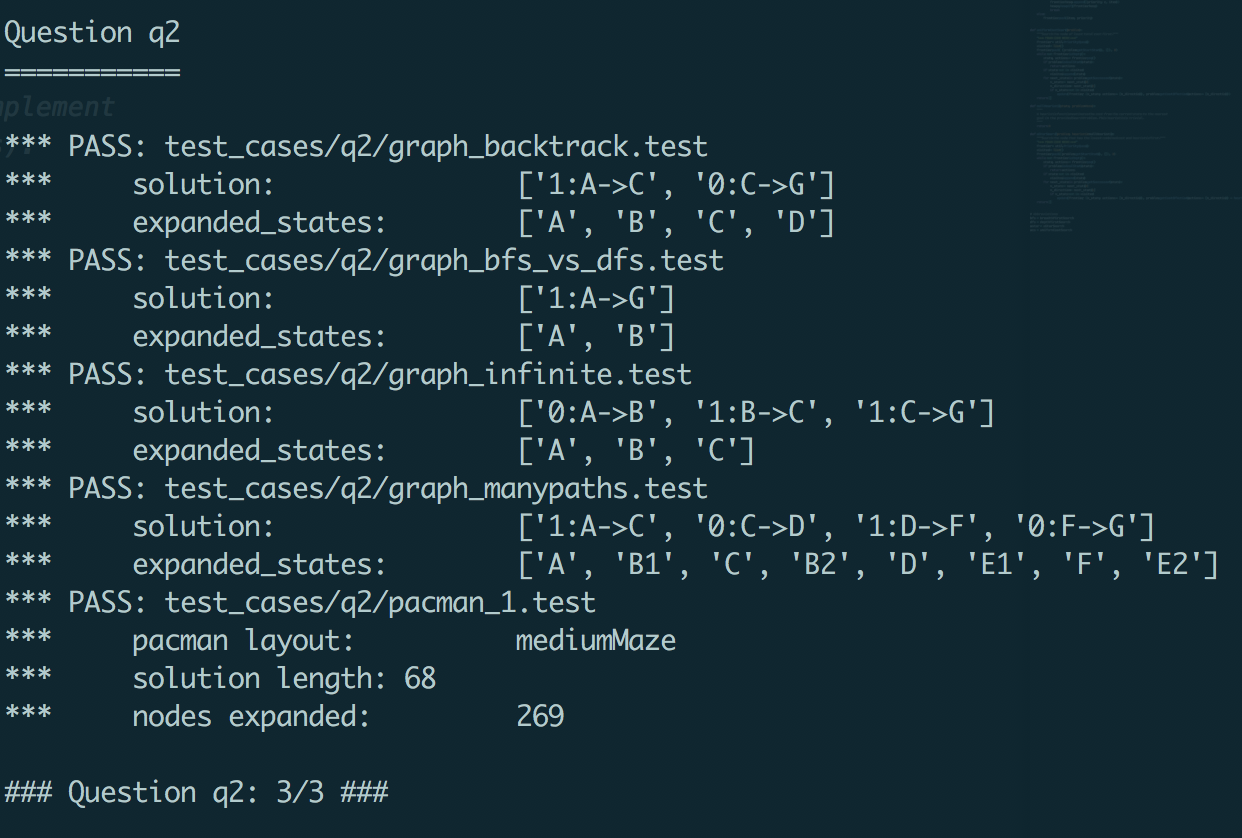
\includegraphics[width=6cm]{q2.png}
\caption{BFS样例测试}
\label{bfs_p1}
\end{minipage}
\begin{minipage}[t]{0.3\textwidth}
\centering
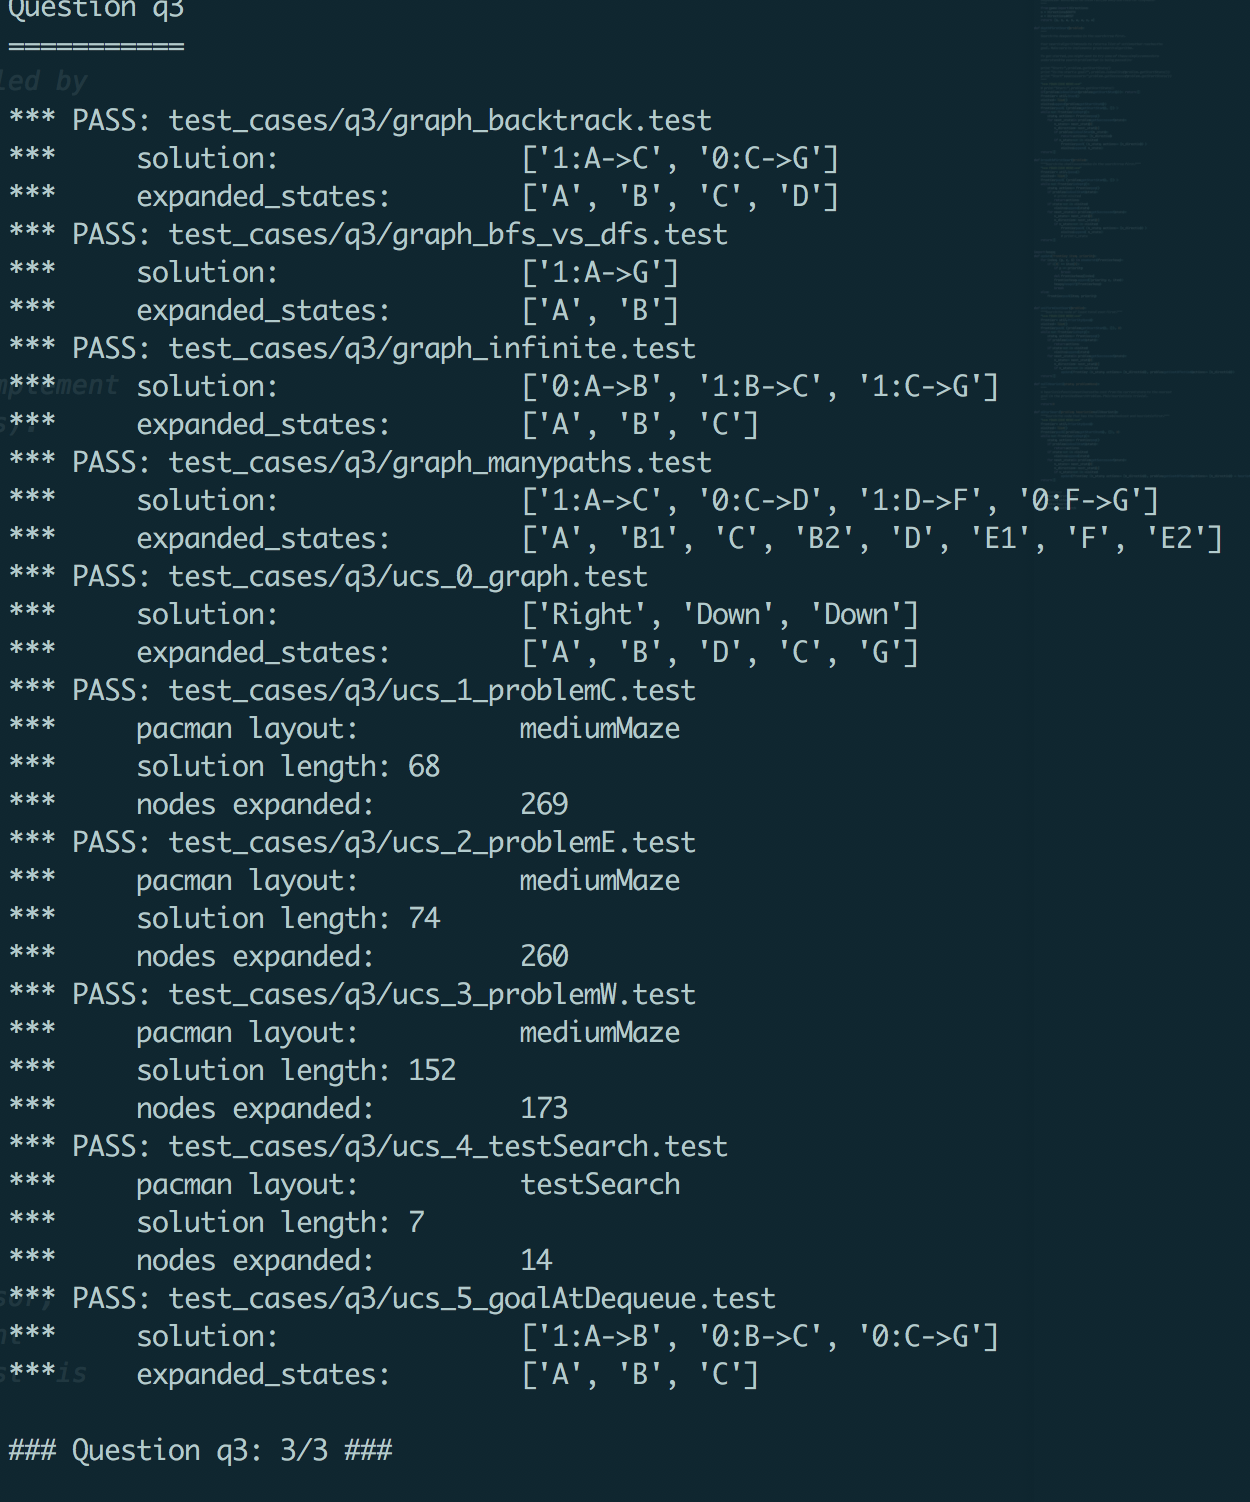
\includegraphics[width=6cm]{q3.png}
\caption{UCS样例测试}
\label{ucs_p1}
\end{minipage}
\begin{minipage}[t]{0.3\textwidth}
\centering
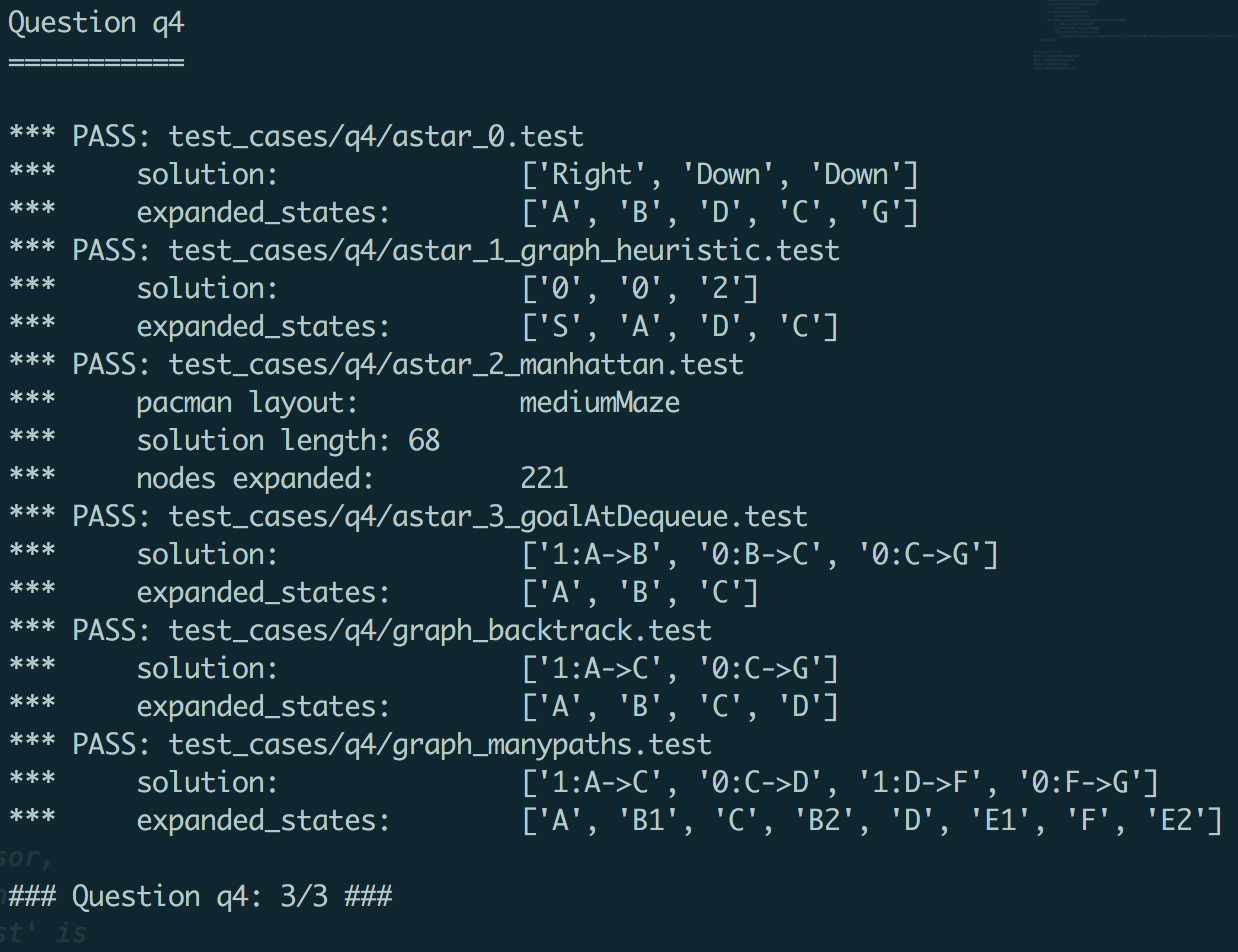
\includegraphics[width=6cm]{q4.png}
\caption{A*样例测试}
\label{A*_p1}
\end{minipage}
\end{figure}

\begin{figure}
\centering
\begin{minipage}[t]{0.48\textwidth}
\centering
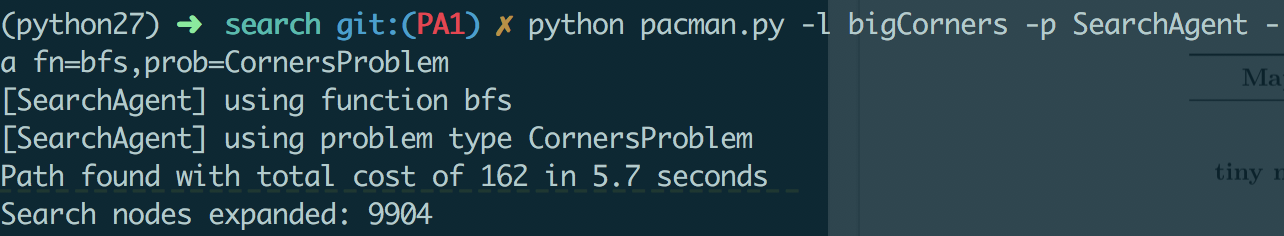
\includegraphics[width=6cm]{bfs_corner.png}
\caption{BFS搜索所有角落}
\label{bfs_p2}
\end{minipage}
\begin{minipage}[t]{0.48\textwidth}
\centering
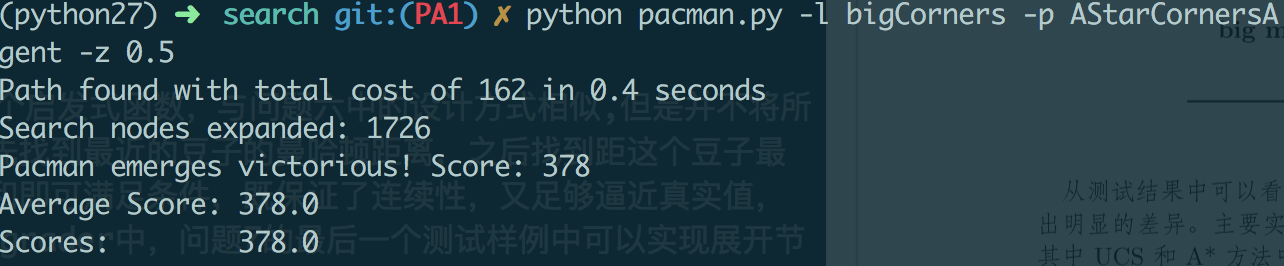
\includegraphics[width=6cm]{astar_corner.png}
\caption{A*搜索所有角落}
\label{astar_p1}
\end{minipage}
\end{figure}





\end{homeworkProblem}

%----------------------------------------------------------------------------------------
%	PROBLEM 2
%----------------------------------------------------------------------------------------

\begin{homeworkProblem}
寻找角落包含下面两个问题:\\
1. Finding All the Corners\\
2. Corners Problem: Heuristic\\

\paragraph{}
问题需要找到所有的角落,需要对返回的数据结构进行修改,记录已经访问的角落,在返回的state中添加对角落的标记之后仿照之前的结构对isGoalState进行修改,就可以完成任务。在启发式函数的设计中,采用将所处位置和剩余角落之间连线的最小曼哈顿距离表示,既可以满足连续性,又可以满足较好的接近真实距离,从而减少了对多余节点的访问,具有较好的性能体现。


\end{homeworkProblem}

%----------------------------------------------------------------------------------------
\begin{homeworkProblem}	
\paragraph{}
吃所有的dots包含以下两个问题:\\
1. Eating All The Dots\\
2. Suboptimal Search\\
\paragraph{}
问题7中需要得到所有的豆子,需要设计一个启发式函数,与问题六中的设计方式相似,但是并不将所有的点连接起来。在设计的算法中,先找到最近的豆子的曼哈顿距离,之后找到距这个豆子最远的豆子的曼哈顿距离,两个距离的和即可满足条件,既保证了连续性,又足够逼近真实值,在测试样例中有较好的体现。在autograder中,问题7的最后一个测试样例中可以实现展开节点数目为8178,如图\ref{q7}
\begin{figure}[ht]
	\centering
	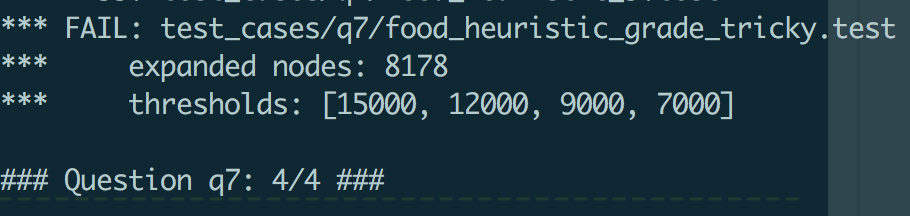
\includegraphics{q7.png}
	\caption{问题7样例测试}
	\label{q7}
\end{figure}
\paragraph{}
问题8中需要使用贪心算法找到最近的豆子并进行线路规划,可以使用bfs进行设计,应该也可以使用ucs进行设计。在程序中实现了bfs设计的算法,可以满足测试样例条件,但是从在地图中的表现中可以看出,这种方式显然不是最优算法,过程中有很多的路程冗余。


\end{homeworkProblem}




\end{document}